
% \vspace{-0.14in}
\section{Data: Solution Augmentation}
\label{sec:data-solution-augmentation}



In this section, we focus on the \emph{Solution Augmentation} part of the \dataset construction pipeline, shown in Figure~\ref{fig:data_overview}. 
We first give a brief overview of how solutions are synthesized for existing questions, and then present ablation studies designed to understand the impact of the different dataset design choices.  

\subsection{Solution Augmentation Preliminaries}
\label{sec:soln_augmentation}
Let $\mathcal{X} = \{\left(q_i, a_i\right)\}_{i=1}^N$ represent a 
typical mathematical reasoning dataset, where $q_i$ and $a_i$ denote the $i^\text{th}$ question and answer respectively. 
To synthesize solutions for this dataset, a \emph{teacher} LLM $\mathcal{M}$ is prompted as follows: 
$$\mathcal{I}\ \left(q_1, s_1\right), \dots, \left(q_K, s_K\right), q'$$ where $\mathcal{I}$ represents the instruction to answer the given math question, $\{q_1, \dots, q_K\}$ represent $K$ questions  representative of the dataset, $\{s_1, \dots, s_K\}$ represent their respective solutions, and $q'$ represents a question from the training set.
Given this prompt, multiple candidate solutions 
are sampled using $\mathcal{M}$. 
The high-quality solutions, usually those that lead to the correct answer, along with the prompt question $q'$, are added to the SFT dataset.



\begin{figure*}[t]
    \centering
    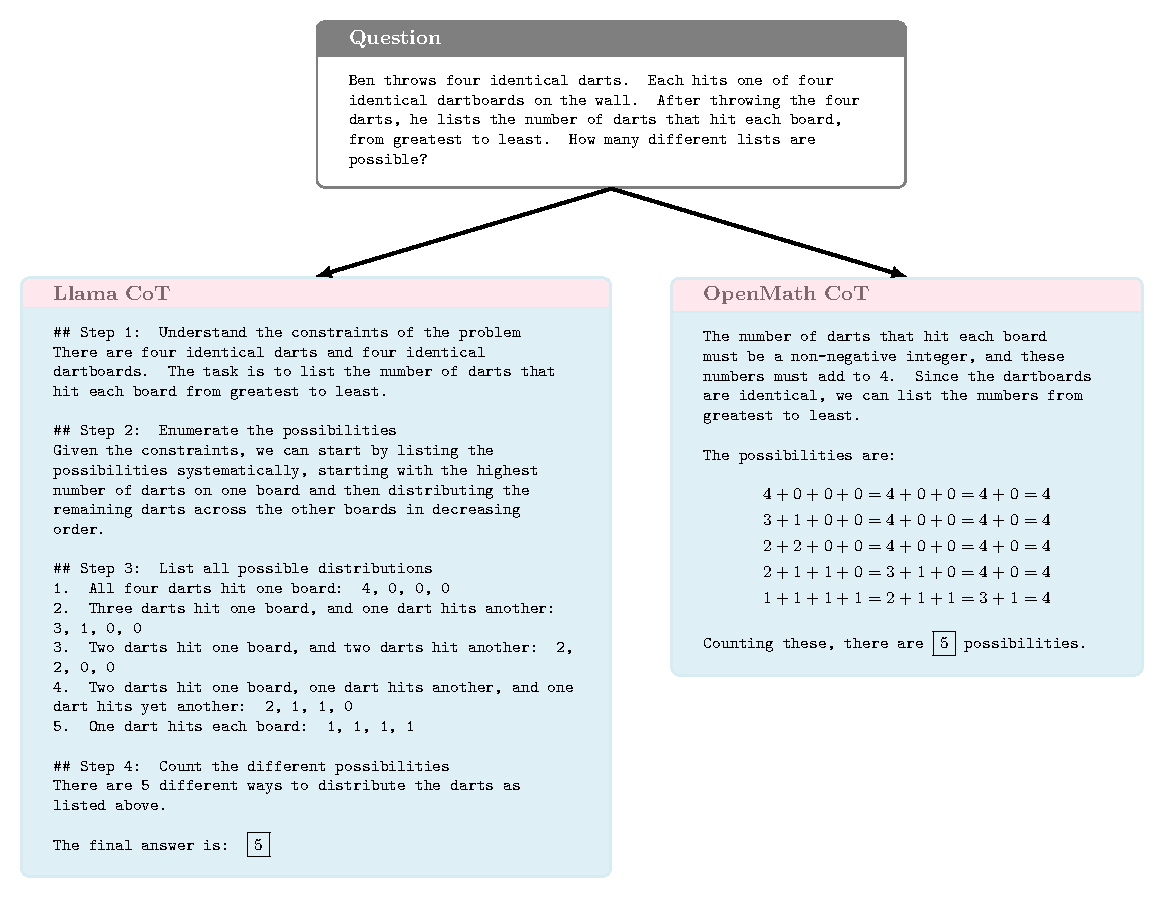
\includegraphics[width=0.95\linewidth]{figures/Solution_Format_Figure.pdf}
    \caption{A sample solution in the Llama CoT format vs.\ the OpenMath CoT format.}
    \label{fig:soln_format}
    % \vspace{-0.1in}
\end{figure*}


\subsection{Ablation Studies}
In the previous section, we gave an abstract overview of the solution augmentation pipeline. 
In practice, several design decisions impact the final SFT dataset, such as the solution format of the few-shot examples $\{s_1, \dots, s_K\}$, the choice of the teacher model $\mathcal{M}$, and the solution filtering mechanism. 
In this section, we study the impact of these different design choices on the SFT performance to guide the dataset construction. 

For these ablation experiments, we use the 1K validation split created from MATH~\citep{hendrycks2021measuringmathematicalproblemsolving} training set by \citet{toshniwal2024openmathinstruct}. The remaining 6.5K MATH training set problems are used to create the SFT dataset. 
The solutions are generated using nucleus sampling~\citep{Holtzman2020The} with a temperature of 1.0 and top-$p$ of 0.95.  
The \texttt{Llama3.1-8B-Base} model is used as the \emph{student} model in all the ablation experiments. 
For SFT, the model is trained for 4 epochs, with a batch size of 256, using the AdamW optimizer~\citep{Loshchilov2019DecoupledWD} with a constant learning rate of 5e-6 and a weight decay of 1e-2. 
To account for the variance in performance across runs, we report the performance averaged across 4 runs.   



\paragraph{Data Downsampling}
For efficiency or experiment design reasons, we sometimes need to downsize an SFT dataset to a specific size or to match another SFT dataset in ablation experiments. We introduce the concept of \emph{coverage} and the two downsampling operations used in the paper.

\emph{Coverage} of a SFT dataset $\mathcal{D}=\{\left(q_i, s_i\right)\}_{i=1}^{T}$ synthesized using dataset $\mathcal{X} = \{\left(q_i, a_i\right)\}_{i=1}^N$ is the fraction of questions in $\mathcal{X}$ with at least one solution in $\mathcal{D}$:
\[ \text{Coverage(}\mathcal{D}, \mathcal{X}\text{)} = \frac{|\{q : \left(q, s\right) \in \mathcal{D}\}|}{|\{q : \left(q, a\right) \in \mathcal{X}\}|} \]


\emph{Fair Downsampling} is a question-dependent downsampling method introduced by~\citet{toshniwal2024openmathinstruct}. 
Due to the varying difficulty of questions, the representation of ``easier'' ones can often dominate an SFT dataset, as generating high-quality solutions for them is ``easier''.  
The goal of \emph{fair} downsampling is to sample question-solution pairs from the original SFT dataset in a way that ensures all questions are as equally represented in the downsampled dataset as possible. 

\emph{Matching Coverage}:
The different design choices explored in the ablation studies result in SFT datasets of varying sizes. 
However, to compare the quality of the datasets, we want to control for the dataset size. 
To this end, we introduce the \emph{Matching Coverage} operation, where SFT datasets are matched at the level of questions. Put simply, after matching coverage, the number of unique questions as well as the number of solutions for each individual question in two dataset is the same.

Formally, suppose we're given two SFT datasets $\mathcal{D}_1$ and $\mathcal{D}_2$. 
Let $Q\left(\mathcal{D}_1\right)$ represent the set of unique questions in $\mathcal{D}_1$:
\[Q\left(\mathcal{D}_1\right) = \{q \mid \left(q, s_1\right) \in \mathcal{D}_1\}\]
The set of common questions in $\mathcal{D}_1$ and $\mathcal{D}_2$ is given by:
\[Q_{\text{match}} = Q\left(\mathcal{D}_1\right) \cap  Q\left(\mathcal{D}_2\right)\]
Let $N\left(\mathcal{D}, q\right)$ represent the number of solutions of question $q$ in dataset $\mathcal{D}$. 
In the matching coverage version of the datasets:
\[
N_\text{match}\left(q\right) = \min\left(N\left(\mathcal{D}_1, q\right), N\left(\mathcal{D}_2, q\right)\right)
\]
for each question $q \in Q_\text{match}$, $N_\text{match}\left(q\right)$ solutions are sampled from the respective datasets.  




This covers the two downsampling methods used in this paper: \emph{Fair Downsampling} and \emph{Matching Coverage}. 
Next, we will describe the ablation experiments.






\subsubsection{Solution Format}


Finetuning with synthetic chain-of-thought (CoT) solutions~\citep{nye2021workscratchpadsintermediatecomputation, wei2022chain, sprague2024cotcotchainofthoughthelps} has been the key to strong performances of small models on math reasoning tasks~\citep{yu2024metamath, toshniwal2024openmathinstruct, dubey2024llama3herdmodels}. 
We find the Llama's CoT format to be quite verbose,\footnote{\url{https://huggingface.co/datasets/meta-llama/Meta-Llama-3.1-8B-Instruct-evals/viewer/Meta-Llama-3.1-8B-Instruct-evals__math__details}} and propose an alternate CoT format, \emph{OpenMath CoT}, which is detailed as well but less verbose. 
Figure~\ref{fig:soln_format} shows a sample solution in the two CoT formats. 

\begin{table*}[t]
\setlength{\tabcolsep}{4pt}
    \centering
    \caption{Comparison of Llama and OpenMath CoT formats on MATH validation accuracy and average solution length measured in number of tokens. }
    \label{tab:soln_format}
    \begin{tabular}{lcc}
    \toprule

 &  MATH Validation Accuracy  &  Mean Solution Length  \\\midrule
Llama CoT       & 40.6 $\pm$ 0.6 & 331.3   \\
OpenMath CoT    & 44.5 $\pm$ 0.8  & 237.0  \\ 
\bottomrule 
    \end{tabular}
\end{table*}



To compare the two CoT formats, we generate SFT data using the \texttt{Llama3.1-405B-Instruct} model. 
For generating solutions in the Llama CoT format we simply use the zero-shot prompt setup as the model was trained on those kinds of solutions. 
However, even when prompting the model with few-shot OpenMath CoT solutions, a substantial number of generations -- 57\% in our experiment -- still follow the Llama CoT format. 
This tendency of \emph{aligned} models reverting to their trained behavior when encountering inputs seen during training has also been observed in prior work~\citep{min-etal-2022-rethinking}. 
We find an interesting workaround to this issue by dropping the special tokens used by Llama-Instruct models. 
Prompting the model with the ``base'' template leads to a dramatic increase in adherence to the OpenMath CoT format and reduces the Llama CoT format generations to only 0.1\%. See Appendix~\ref{sec:app_soln_format} for the prompt and more details. 







With 64 solutions sampled per question, the zero-shot setup results in about 30\% more solutions than the few-shot prompt setup (350K vs 268K). 
To control for the confounding factor of SFT data size, we perform the Matching Coverage operation over the two datasets which reduces the final SFT dataset to 260K question-solution pairs. 
Table~\ref{tab:soln_format} shows that the OpenMath CoT format is 40\% less verbose than the Llama CoT format and also results in a better SFT performance. 
All experiments presented henceforth use the OpenMath CoT format. 

    
    
    
    








\subsubsection{Choice of Teacher Model}
\label{sec:teacher_model}


Prior work has shown that with repeated sampling, even weak models can match or outperform much stronger/bigger models~\citep{li2024common7blanguagemodels, brown2024largelanguagemonkeysscaling}. 
In fact, for a fixed compute budget, a weaker model can be a better choice for a teacher model~\citep{bansal2024smallerweakerbettertraining}. 
But data synthesis is a one-time expense and a small portion of the overall compute budget of training LLMs~\citep{epoch2023tradingoffcomputeintrainingandinference}. 
We instead ask the following question: 
\emph{Can a student model learn better from its own generated solutions vs solutions generated by a strong teacher model when matching the SFT data coverage?}
\begin{table*}[t]
    \setlength{\tabcolsep}{4pt}
    \centering
    \caption{\texttt{Llama3.1-8B-Base} vs.\ \texttt{Llama3.1-405B-Instruct} as data generation models. 
    }
    \begin{tabular}{lcc}
    \toprule
        &   MATH Validation Accuracy &  Mean Solution Length \\ \midrule
    Llama3.1-8B-Base & 30.1 $\pm$ 0.6  & 205.7 \\ 
    Llama3.1-405B-Instruct & 37.9 $\pm$ 0.6 & 180.2 \\ 
    
\bottomrule 
    \end{tabular}
    \label{tab:teacher_model}
    % \vspace{-0.1in}
\end{table*}


In this ablation, we compare \texttt{Llama3.1-8B-Base} and \texttt{Llama3.1-405B-Instruct} as teacher models.  
We sample solutions using the two models and perform the Matching Coverage operation to match the final SFT datasets precisely. 
The SFT results presented in Table~\ref{tab:teacher_model}  show that even when controlling for the SFT data size, \texttt{Llama3.1-405B-Instruct} is a far superior data generation model. 
Our preliminary analysis suggests that the reason is weaker models generate more  \emph{noisy solutions} that use incorrect reasoning yet end up with the right answer and, ultimately, part of the SFT dataset (Appendix~\ref{sec:app_noisy_solutions}).  
We leave a more detailed analysis regarding this for future work.  
Next, we investigate the impact of these \emph{noisy solutions} among solutions generated by \texttt{Llama3.1-405B-Instruct}. 




\subsubsection{Impact of Low-Quality Solutions}
\label{sec:impact-of-noise}
\begin{table*}[!ht]
    \centering
    \caption{SFT performance on the MATH validation set with various filtering strategies to remove solutions with incorrect reasoning.}
    \label{tab:nosiy-data-sft-performance}
    \begin{tabular}{lcc}
    \toprule
     Filtering Strategy    &  Data Size & MATH Validation Accuracy \\ \midrule
     Unfiltered      & 128K &  43.6 $\pm$  1.7 \\
     LLM-as-a-Judge: Prompt 1 & 113K           &  43.6 $\pm$ 0.1 \\ 
     LLM-as-a-Judge: Prompt 2  & 116K          &  43.0 $\pm$
     0.8  
     \\
     Nemotron-4-340B-Reward: Helpfulness $\ge 3$             &  118K &  43.8 $\pm$ 0.4 \\
     Nemotron-4-340B-Reward: Correctness $\ge 3$  &  120K &  43.1 $\pm$ 0.4 
     \\  \bottomrule
    \end{tabular}
\end{table*}



Data quality plays an important role in the accuracy of LLMs~\citep{jain2024llmassisted}.  
We explore the impact of data quality on the final SFT performance in our setup. 
First, we employ automated LLM-based methods to filter out solutions that, despite reaching the correct answer, use incorrect reasoning. Second, we investigate the effects of intentionally incorporating incorrect solutions into the SFT dataset.


\paragraph{Removing Low-Quality Solutions.}
Synthetic solutions produced in our pipeline may include examples where the intermediate steps are incorrect, yet still lead to the right final answer.
For simplicity, we refer to these instances as ``low-quality'' data.  In this section, we will discuss how we identify and remove low-quality data, followed by an investigation into its impact on the SFT performance.

We employ two methods to identify low-quality data: LLM-as-a-Judge and reward model. In the LLM-as-a-Judge approach, we design two  prompts for the \texttt{Llama3.1-405B-Instruct} to determine whether the generated solutions contain incorrect intermediate steps, providing a binary outcome (see Appendix \ref{sec:LLM-as-a-judge-prompt} for the prompts). For the reward model labeling method, we use Nemotron-4-340B-Reward \citep{wang2024helpsteer2} to evaluate the quality of the generated solutions based on factors like helpfulness (the overall usefulness of the response to the prompt) and correctness (the inclusion of all relevant facts without errors). Helpfulness and correctness are rated on a scale from 0 to 4, where a higher score indicates better data quality. For the reward model filtering, we used a threshold of 3 based on small-scale tuning experiments. 

To determine the impact of filtering low-quality data on the SFT performance, we use a 128K-sized fair downsampled SFT dataset. 
We call this \emph{Unfiltered} data and use a model trained on it as a baseline. 


Table \ref{tab:nosiy-data-sft-performance} presents the statistics of data remaining with different filtering approaches, and the corresponding SFT performance. 
The proportion of data filtered by the different methods ranges from 6\% to 12\%, a non-negligible fraction of the overall data. \footnote{Our manual analysis of 20 examples identified by the two approaches suggests that approximately 60\% of the solutions are indeed incorrect.}
Yet none of the filtering strategies give any meaningful gain over the baseline \emph{Unfiltered} model. 
This means that either SFT is robust to the presence of up to 10\% of low-quality solutions or our filtering is not accurate enough. We investigate this question next.


\begin{figure*}[ht]
    \centering
    \begin{subfigure}[b]{0.45\textwidth}
        \captionsetup{justification=centering}
        \centering
        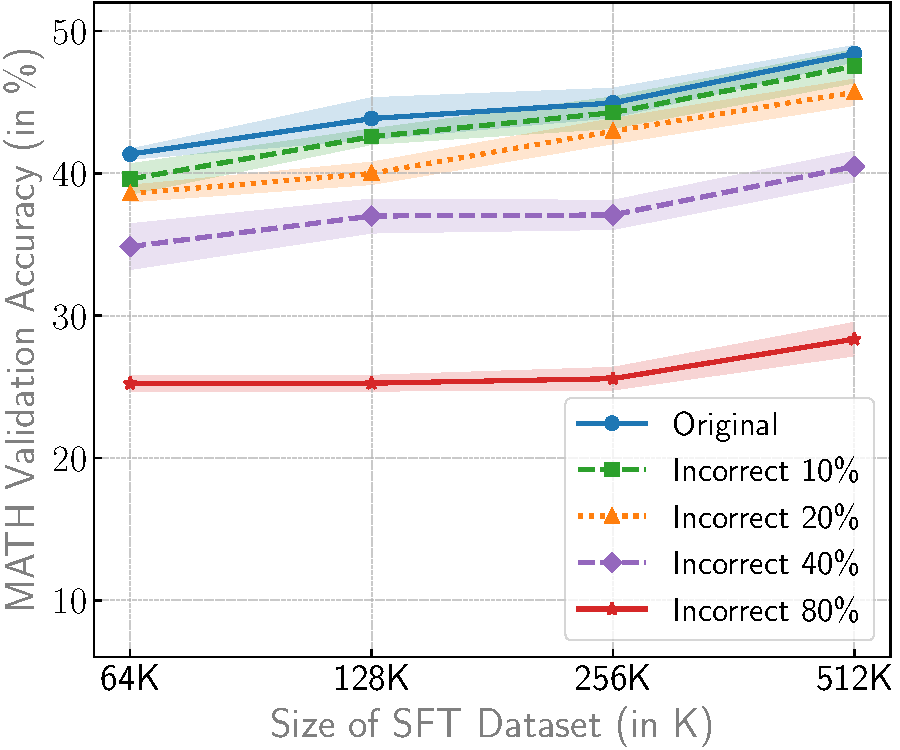
\includegraphics[width=\textwidth]{plots/noise_solution_with_err_bar.pdf}  %
        \caption{Adding wrong-answer solutions.}
        \label{fig:figure1}
    \end{subfigure}
    \hfill
    \begin{subfigure}[b]{0.45\textwidth}
    \captionsetup{justification=centering}
        \centering
        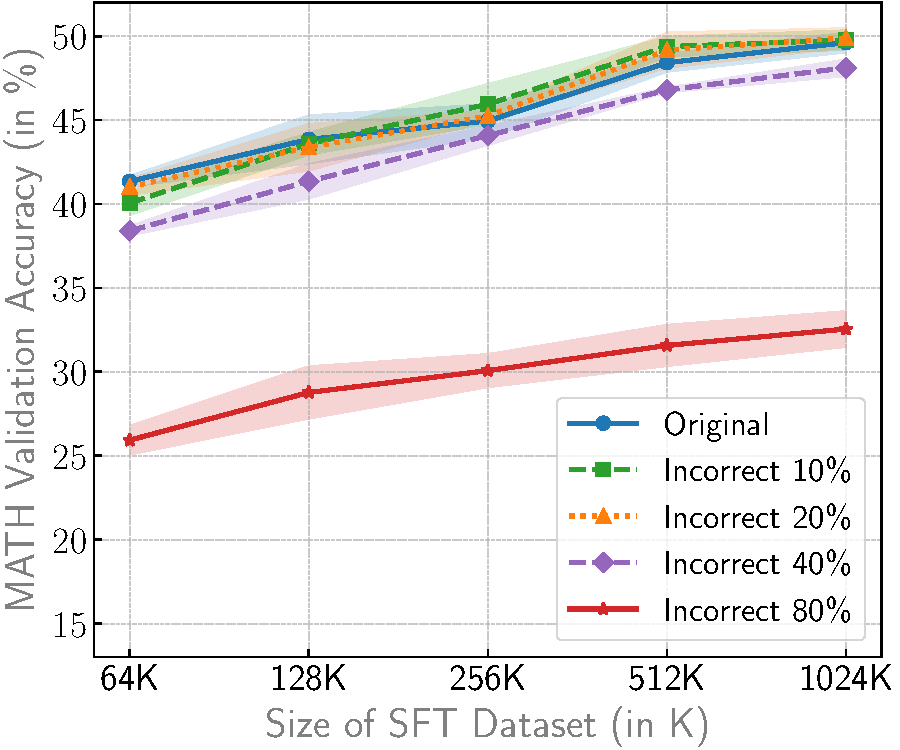
\includegraphics[width=\textwidth]{plots/noise_pairing_with_err_bar.pdf}  %
        \caption{Correct solutions mismatched with questions}
        \label{fig:figure2}
    \end{subfigure}
    
    \captionsetup{justification=centering}\caption{Impact of low-quality solutions on the SFT performance. }
    % \vspace{-0.2in}
    \label{fig:incorrect_solutions}
\end{figure*}









\paragraph{Adding Low-Quality Solutions.}


In the previous section, we see that filtering low-quality solutions generated by a strong model such as \texttt{Llama3.1-405B-Instruct} leads to almost the same or worse SFT performance in comparison to no filtering. 
While our manual analysis suggests that most of the filtered out solutions were indeed using incorrect reasoning, the automatic filtering approaches are far from perfect and it's hard to gauge the impact of filtering out correct solutions which have been classified as incorrect. 

To remove the effect of potentially inaccurate filtering, we can instead study the impact of explicitly adding low-quality/incorrect solutions on the SFT performance. 
We consider two strategies of adding ``bad'' solutions:
\begin{enumerate}
    \item \textbf{Wrong-answer Solutions}: By incorporating solutions generated by the teacher LLM, which were excluded during the creation of the SFT dataset due to not arriving at the ground truth answer.
    \item \textbf{Incorrect Pairing}: 
    By shuffling some of the question-solution pairs in the SFT dataset, such that the correct solutions are paired with unrelated questions.  
\end{enumerate}

For both these strategies, we experiment with varying the proportion of such incorrect solutions from \{10\%, 20\%, 40\%, 80\%\}. 
We also vary the SFT data size from  \{64K, 128K, 256K, 512K, 1024K\} to study the impact on SFT performance at different data scales\footnote{For the ``Wrong-answer Solutions'' setting, we were not able to run the experiments for 1024K data size because the \texttt{Llama3.1-405B-Instruct} model makes few mistakes on the MATH training set.}.  

Figure~\ref{fig:incorrect_solutions} presents the impact of incorrect solutions on the SFT performance at varying data sizes. 
From both the plots we see that the model performance suffers little to no performance degradation with as much as 20\% incorrect solutions at data scales $\ge 256$K. Among the two strategies, we see that the model is especially robust to ``Incorrect Pairing'' with strong performance even with 40\% incorrect solutions. 

Based on these results we conclude that models are indeed robust to the presence of up-to 20\% of low-quality solutions during SFT and extensive data filtering at this stage has limited gains.

\subsubsection{Impact of Question Diversity}


To investigate the impact of question diversity on SFT performance, we construct finetuning datasets with 256K question-solution pairs with the number of unique questions varying from \{1K, 2K, 4K, 6.5K\}. Figure~\ref{fig:question_diversity} shows a clear trend that the SFT performance improves with an increase in the number of unique questions, with a drop of more than 10 points when the number of unique questions is limited to 1K. 
This result highlights the potential of generating new questions, and we describe the Question-Solution Augmentation pipeline next. 


\begin{figure}
    \centering
    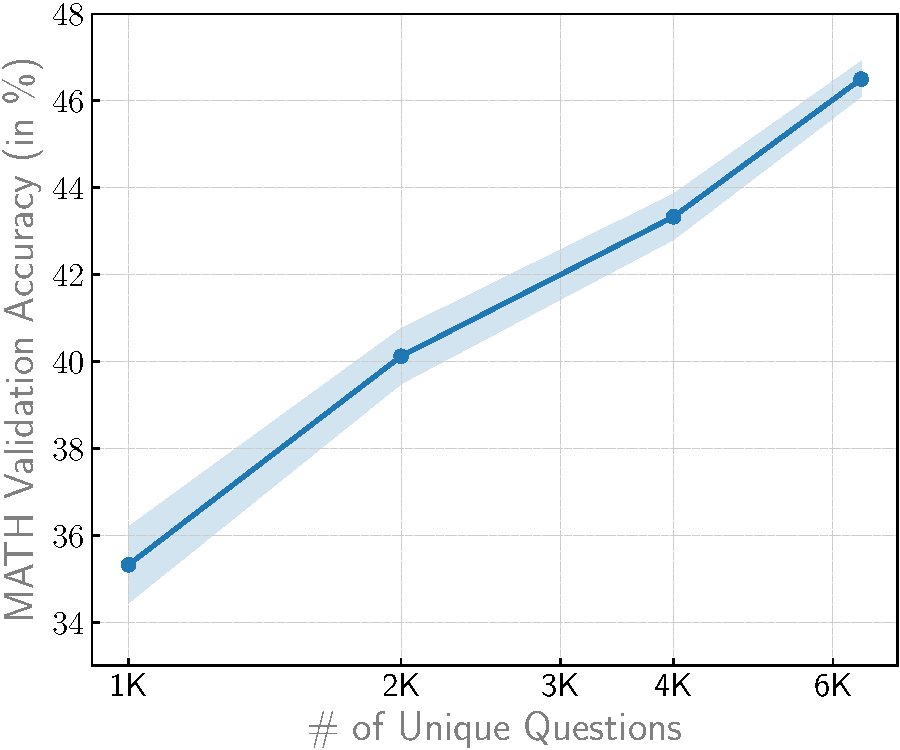
\includegraphics[width=0.85\linewidth]{plots/question_diversity.pdf}
    \caption{Impact of question diversity on MATH validation accuracy.} 
    \label{fig:question_diversity}
    \vspace{-0.2in}
\end{figure}



 



